\renewcommand{\chaptername}{March 15th: Lab}
\chapter{Quantum Teleportation}
In quantum teleportation, the properties of quantum entanglement are used to send a qubit between observers without physically moving the involved qubit. The qubits themselves are not really teleported, but the state of one qubit is destroyed on one side and extracted on the other side, so the information that the state encodes is communicated. The usefulness of quantum teleportation lies in its ability to send quantum information arbitrarily far distances without exposing quantum states to thermal decoherence from the environment or other adverse effects.
%The number of entangled states necessary to accomplish this is well outside anything physically achievable, since maintaining such a massive number of entangled states without decohering is a difficult problem.

\section{Method}

The following qubit state  $|\Psi \rangle = \alpha |0 \rangle + \beta |1 \rangle$ needs to be transferred. By taking advantage of two classical bits and an entangled qubit pair, the state $|\Psi \rangle$ can be transferred.

The following steps were followed to create an entanglement protocol and to perform quantum teleportation.

\begin{enumerate}
    \item Use a third party entangled qubit pair
    \item Perform operations on the qubit that must be sent
    \item Send the results over a classical communication channel
    \item Perform some operations on the received information to receive the qubit
\end{enumerate}

\section{Results}

\subsubsection{Step 1}
q1 and q2 were entangled together to be used as an entangled pair.
\begin{figure}[h]
\centering
\begin{tabular}{c}
\begin{minipage}[c]{.45\linewidth}
\begin{minted}[fontsize=\small
frame=lines,
framesep=2mm,
baselinestretch=1.2,
bgcolor=LightGray,
fontsize=\footnotesize,
linenos
]{python}
q = QuantumCircuit(4,2)

psi = random_statevector(2)
q.append(Initialize(psi), [0])

q.cx(0,1)
q.h(0)

q.draw(output='mpl')
\end{minted}
\end{minipage}
\begin{minipage}[c]{.1\linewidth}
\centering
$\rightarrow$
\end{minipage}
\begin{minipage}[c]{.4\linewidth}
\centering
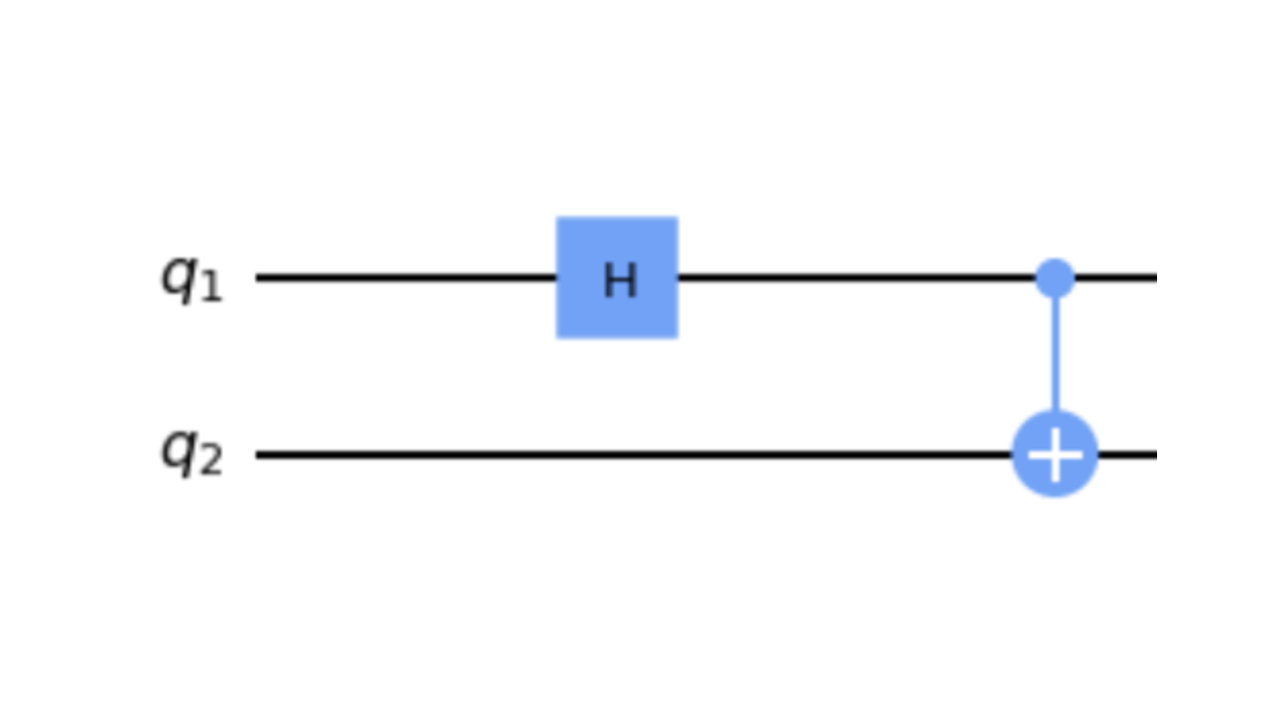
\includegraphics[width=\textwidth]{lab3/images/Step1.png}
\end{minipage}\\
\\ %empty line for some space
\end{tabular}
\caption{Code and circuit diagram to produce entangled pair}
\label{step1}
\end{figure}

Python library with tools to facilitate simulation of quantum systems

\subsubsection{Step 2}
Backwards enanglement thing

\begin{figure}[h]
\centering
\begin{tabular}{c}
\begin{minipage}[c]{.45\linewidth}
\begin{minted}[fontsize=\small
frame=lines,
framesep=2mm,
baselinestretch=1.2,
bgcolor=LightGray,
fontsize=\footnotesize,
linenos
]{python}
q = QuantumCircuit(4,2)

psi = random_statevector(2)
q.append(Initialize(psi), [0])

q.cx(0,1)
q.h(0)

q.draw(output='mpl')
\end{minted}
\end{minipage}
\begin{minipage}[c]{.1\linewidth}
\centering
$\rightarrow$
\end{minipage}
\begin{minipage}[c]{.4\linewidth}
\centering
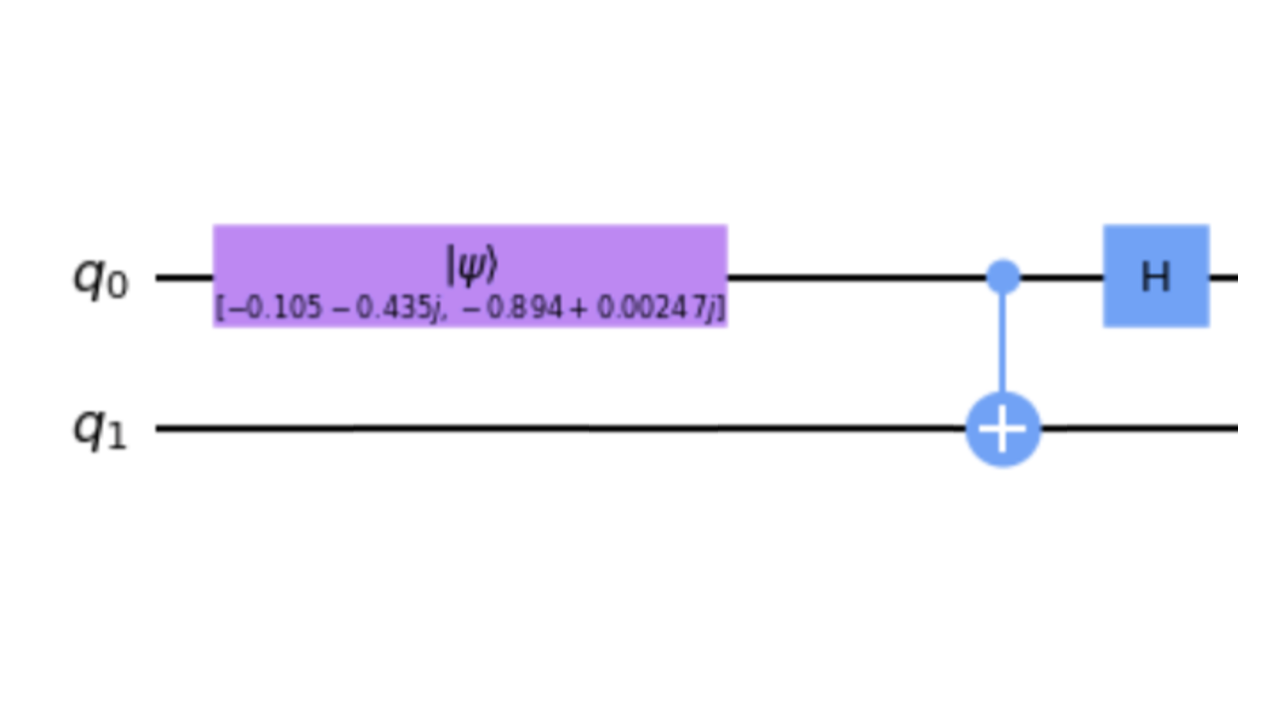
\includegraphics[width=\textwidth]{lab3/images/Step2.png}
\end{minipage}\\
\\ %empty line for some space
\end{tabular}
\caption{Main caption}
\label{step2}
\end{figure}


\subsubsection{Step 3}
Measure

\begin{figure}[h]
\centering
\begin{tabular}{c}
\begin{minipage}[c]{.45\linewidth}
\begin{minted}[fontsize=\small
frame=lines,
framesep=2mm,
baselinestretch=1.2,
bgcolor=LightGray,
fontsize=\footnotesize,
linenos
]{python}
q = QuantumCircuit(4,2)

psi = random_statevector(2)
q.append(Initialize(psi), [0])

q.cx(0,1)
q.h(0)

q.draw(output='mpl')
\end{minted}
\end{minipage}
\begin{minipage}[c]{.1\linewidth}
\centering
$\rightarrow$
\end{minipage}
\begin{minipage}[c]{.4\linewidth}
\centering
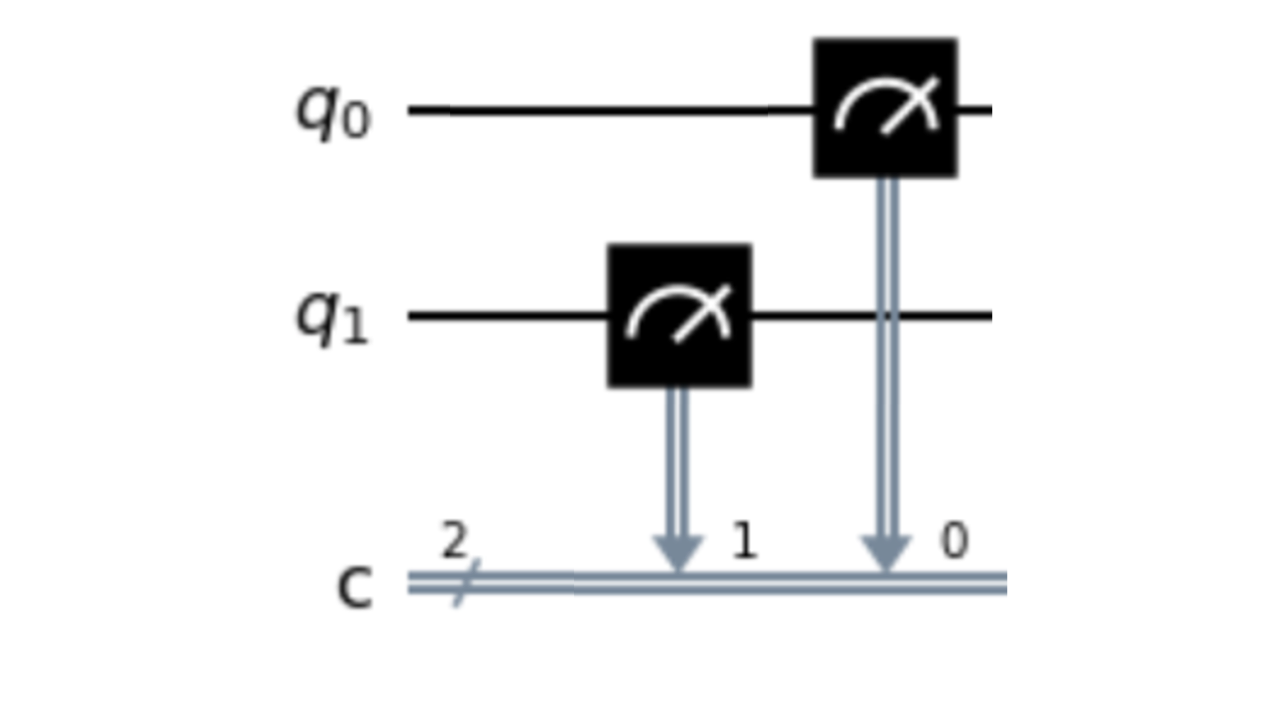
\includegraphics[width=\textwidth]{lab3/images/Step3.png}
\end{minipage}\\
\\ %empty line for some space
\end{tabular}
\caption{Main caption}
\label{step3}
\end{figure}

\subsubsection{Step 4}
The conditions that had to be satisfied
control if gates

\begin{figure}[h]
\centering
\begin{tabular}{c}
\begin{minipage}[c]{.45\linewidth}
\begin{minted}[fontsize=\small
frame=lines,
framesep=2mm,
baselinestretch=1.2,
bgcolor=LightGray,
fontsize=\footnotesize,
linenos
]{python}
q = QuantumCircuit(4,2)

psi = random_statevector(2)
q.append(Initialize(psi), [0])

q.cx(0,1)
q.h(0)

q.draw(output='mpl')
\end{minted}
\end{minipage}
\begin{minipage}[c]{.1\linewidth}
\centering
$\rightarrow$
\end{minipage}
\begin{minipage}[c]{.4\linewidth}
\centering
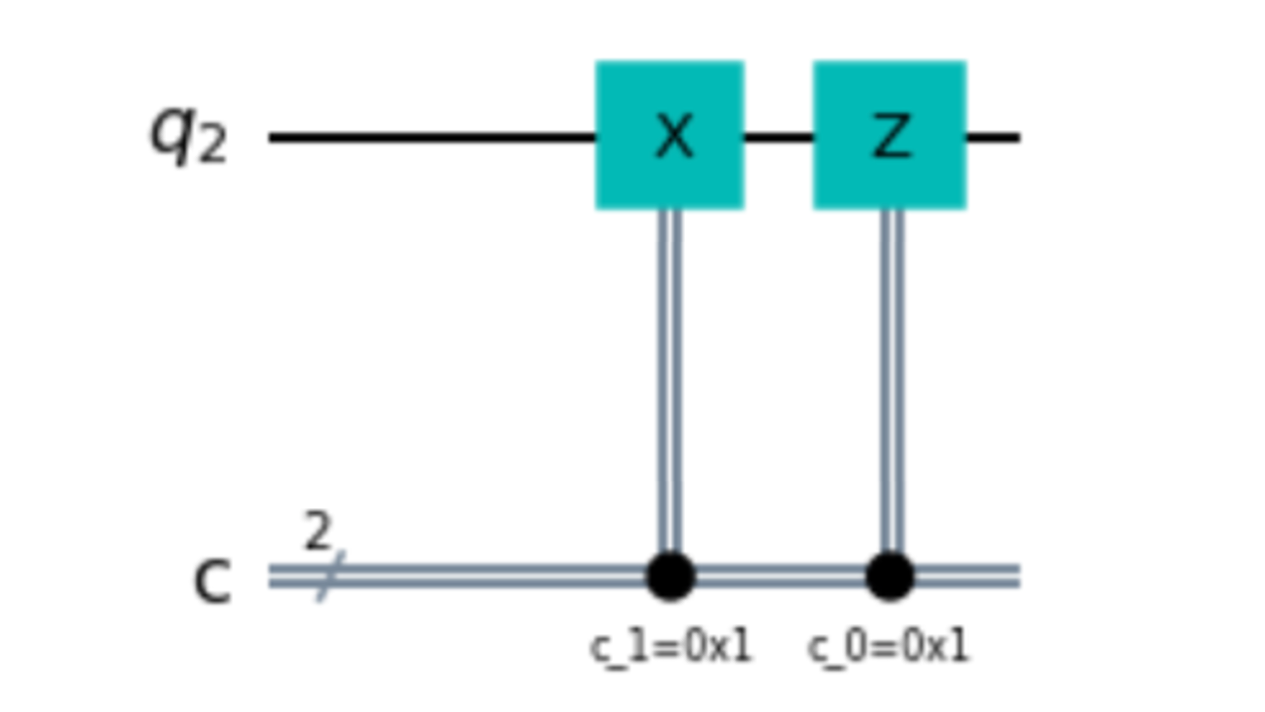
\includegraphics[width=\textwidth]{lab3/images/Step4.png}
\end{minipage}\\
\\ %empty line for some space
\end{tabular}
\caption{Main caption}
\label{step4}
\end{figure}

\subsubsection{Final Design}
The circuit written to perform `quantum teleportation' is shown in Figure \ref{fig:teleportCircuit}.
\begin{figure}[h]
    \centering
    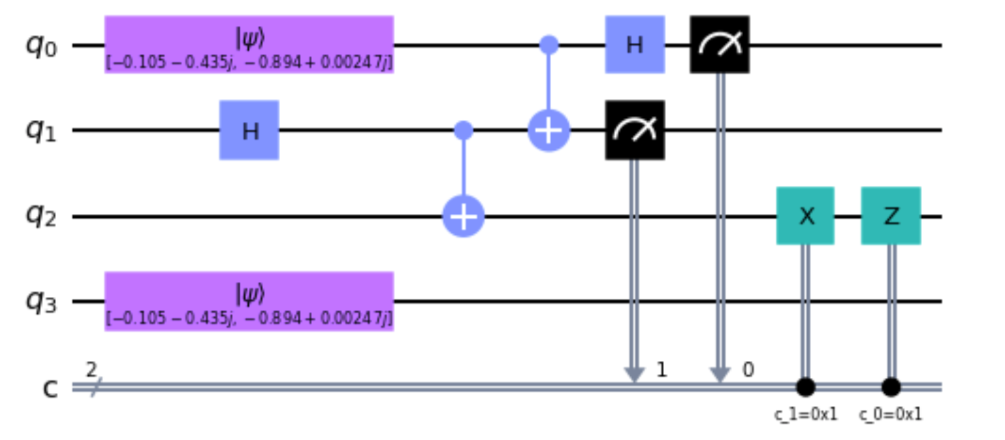
\includegraphics[width=0.6\textwidth]{lab3/images/teleportCircuit.png}
    \caption{teleportCircuit}
    \label{fig:teleportCircuit}
\end{figure}

The result from this circuit was observed using Bloch Sphere representation, as seen in Figure \ref{fig:teleportBloch}
\begin{figure}[h]
    \centering
    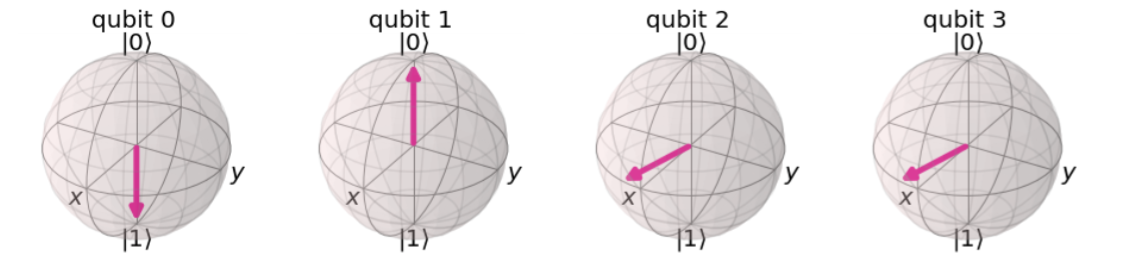
\includegraphics[width=\textwidth]{lab3/images/teleportBloch.png}
    \caption{Bloch sphere showing the state of each qubit after teleportation has occurred}
    \label{fig:teleportBloch}
\end{figure}

Qubit 3 was initialised to be the same as qubit 0 (the qubit that is being `quantum-ly teleported'). This was done purely to ensure the same qubit was extracted. Qubit 2 is the qubit that was extracted after teleportation. It is clear that it is the same as qubit 3, thus proving the circuit worked. To verify the robustness of this design, the circuit was built using IBMs remote quantum computer. The result from which can be seen in Figure \ref{fig:ibmTeleport} and are discussed in Section \ref{sec:discussTeleport}.
\begin{figure}[h]
    \centering
    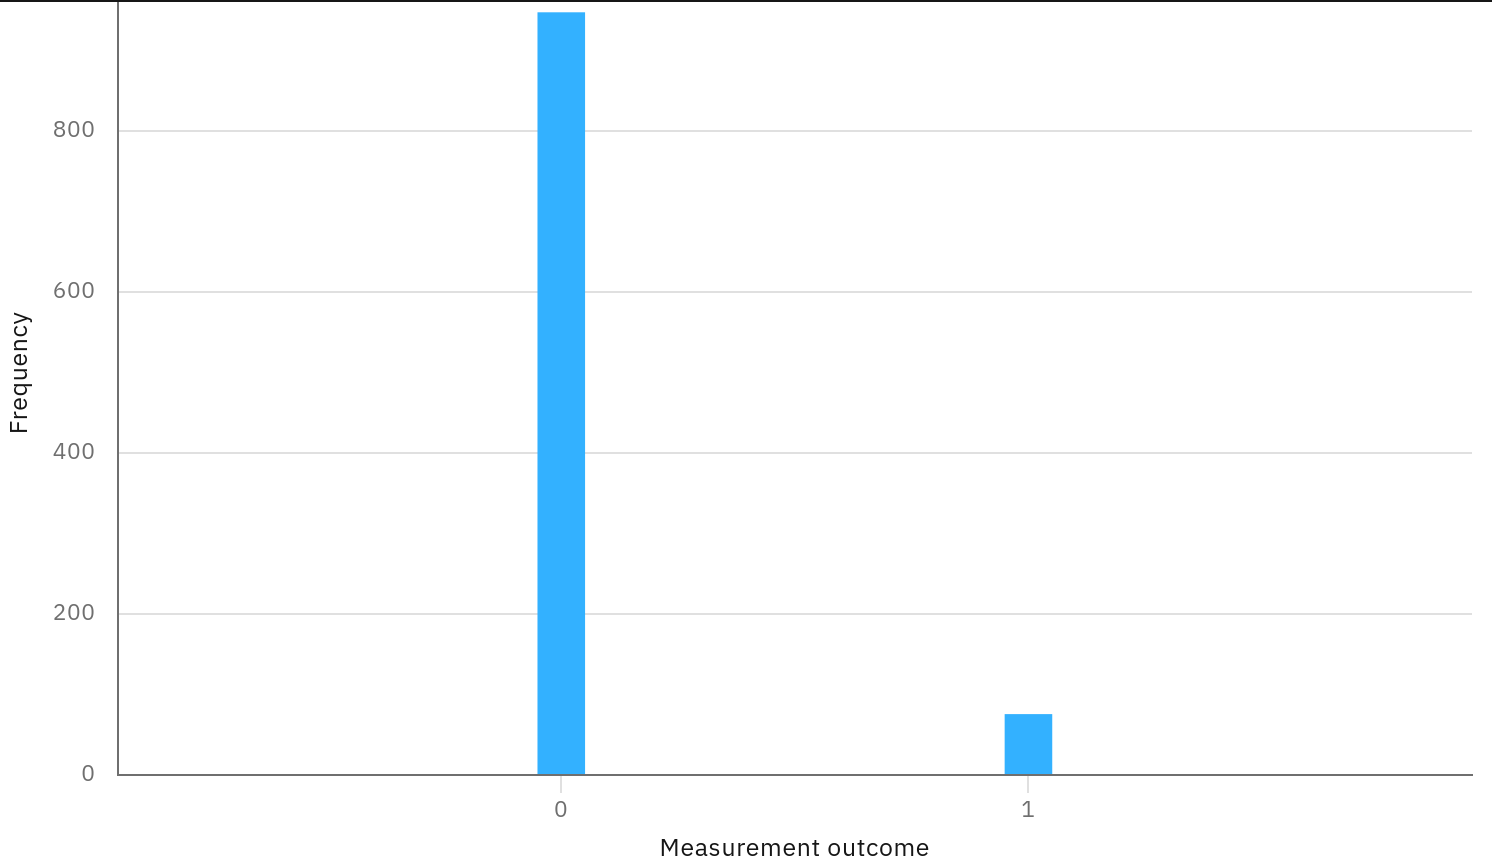
\includegraphics[width=0.38\textwidth]{lab3/images/ibmTeleport.png}
    \caption{Histogram showing measurement outcome \textbf{after teleportation}}
    \label{fig:ibmTeleport}
\end{figure}

\section{Comparison of results with theory}
\section{Discussion} \label{sec:discussTeleport}
\textbf{Question 1:}

Follow the steps above, and the knowledge of qiskit you now have from Lab 2 to create an entanglement protocol. You may also benefit from the little revision above which introduce a couple of new features of qiskit

\textbf{Question 2:}

\textbf{2(a)}: Use IBM composer and compare its results to what you obtained above. Are they different? How so?

Its in format output state = q0 q1 q2

\textbf{2(b):} Now that you have implemented it, what could quantum teleportation be used for and why is it important?

\section{Conclusions}

\begin{itemize}
    \item Implement a quantum algorithm
    \item Understand the principles on quantum teleportation and how it can be implemented/applied
\end{itemize}